\documentclass{article}
\usepackage[margin=0.5in]{geometry}
\usepackage{graphicx}
\usepackage{wrapfig}
\usepackage{amsmath}
\graphicspath{{Images/Appendix/Hough/}}
\usepackage[ampersand]{easylist}

\begin{document}
	
	\title{A brief overview of a simple approach to lane detection}
	\author{Michael McDonnell}
	\date{}
	\maketitle
	
%	\begin{abstract}
%		The abstract text goes here.
%	\end{abstract}
%	
	\section{Overview}
	This document provides an overview of a very simple approach to detecting straight lanes on a road surface. The approach will be outlined in general and basic theory of the supporting concepts will be covered. This is not intended as a standalone document to develop robust lane detection, merely an introduction for the interested reader.
	
%	\begin{equation}
%	\label{simple_equation}
%	\alpha = \sqrt{ \beta }
%	\end{equation}
	
	\subsection{General Approach}
	A basic approach to lane detection using a vehicle mounted camera is as follows:
	\begin{easylist}[itemize]
		& Isolate the area of interest in the frame as the image data to be operated on, \textit{$I$}
		& Convert the pixels in \textit{$I$} from RGB to greyscale, \textit{$I_g$}
		& Identify edge pixels from \textit{$I_g$} using an edge detection algorithm, resulting in a binary edge map, \textit{$E$}
		&& Optionally preprocess image data by low pass filtering (blur) prior
		& Transform the edge pixels, \textit{$E$} into Hough space \textit{$H$}
		& Identify a set of lines of interest \textit{$l$} by thresholding \textit{$H$} to an appropriate level
		& For each lane/road edge, left and right:
		&& From a subset of lines in \textit{$l$} representing lines within an angle of interest for the lane edge (ie. limit the lines to the expected angle range), select the line with the highest value (vote count).
	\end{easylist}

	The end result of this approach, assuming the road lines are adequately marked, is a line either side of the lane representing the approximated lane lines. Note that the above approach did not include inverse perspective mapping. This is a technique that provides a `birds eye view' of the image by transforming the pixels and is commonly used in lane detection however is not required in this simple case.
	
	\section{Isolation of image data \textit{$I$}}
	%\setlength{\columnsep}{0pt}%
	\setlength{\intextsep}{0pt}%
	\begin{wrapfigure}{h!}{0.35\textwidth}
		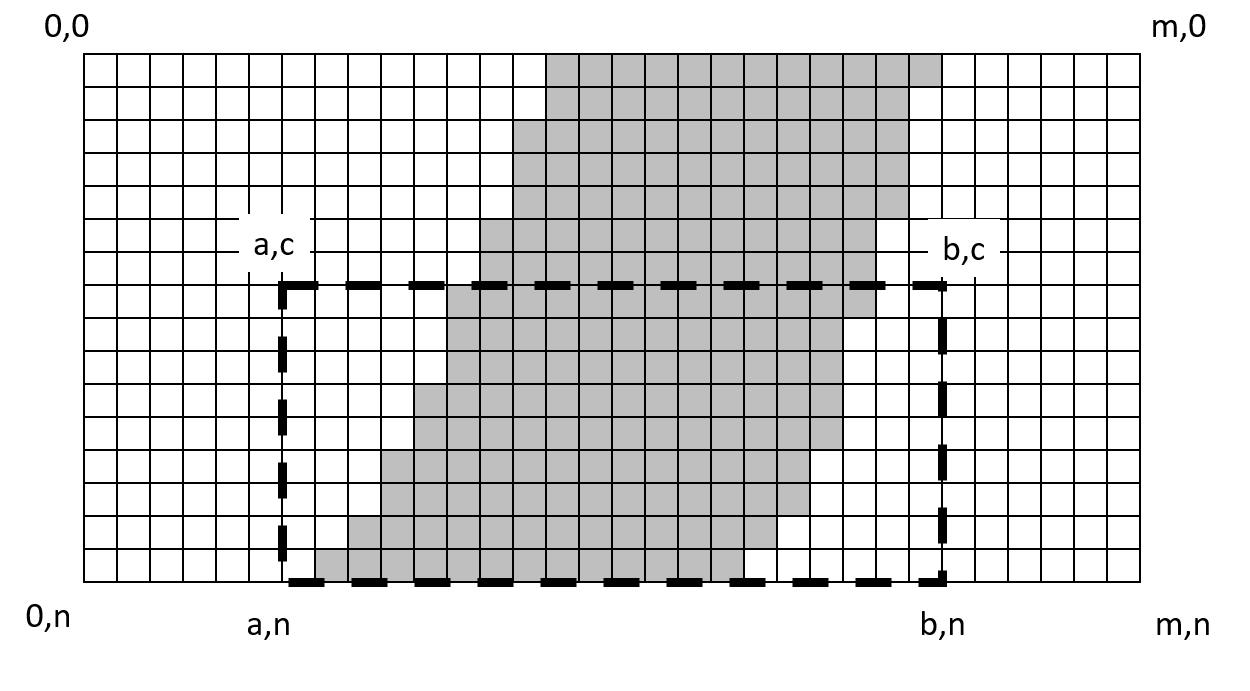
\includegraphics[width=0.34\textwidth]{pixelSubset}
		\caption{Subset of pixels from the full image array}
		\label{pixelSubset}
	\end{wrapfigure}
	
	Image data is stored as a two dimensional array of colours (usually represented by a three element vector for Red, Blue and Green channels). Isolation of the data in the region of interest is as simple as selecting a subrange of the array in the relevant area. A simple example of this is shown in figure \ref{pixelSubset} where the subset from $(a,c)$ to $(b,n)$ is defined as the region of interest. In this case the image data to be operated on, \textit{$I$} would be a new array with the values $(a,c)$ to $(b,n)$. Conversion to greyscale is simply a weighted average of the channels, with different algorithm implementations weighting channels in different ratios.
	
%	\begin{wrapfigure}{r}{0.35\textwidth}
%		\begin{center}
%			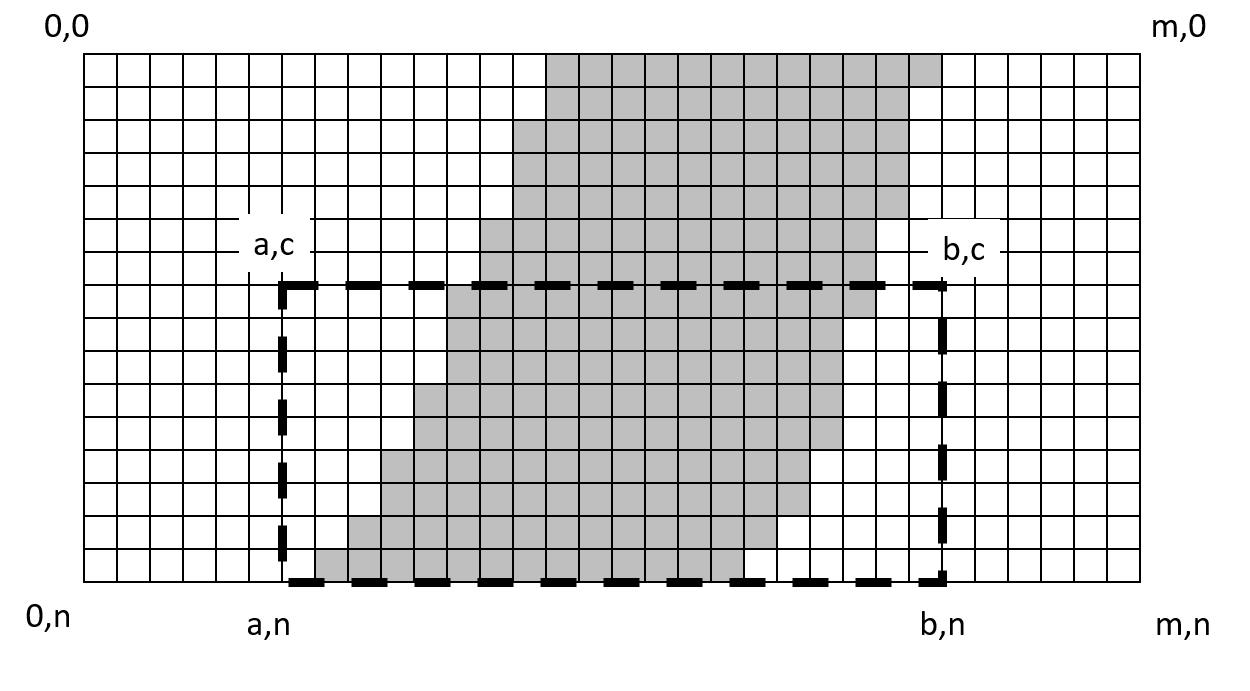
\includegraphics[width=0.34\textwidth]{pixelSubset}
%		\end{center}
%		\caption{Subset of pixels from the full image array}
%		\label{pixelSubset}
%	\end{wrapfigure}



%	\begin{figure}
%		\centering
%		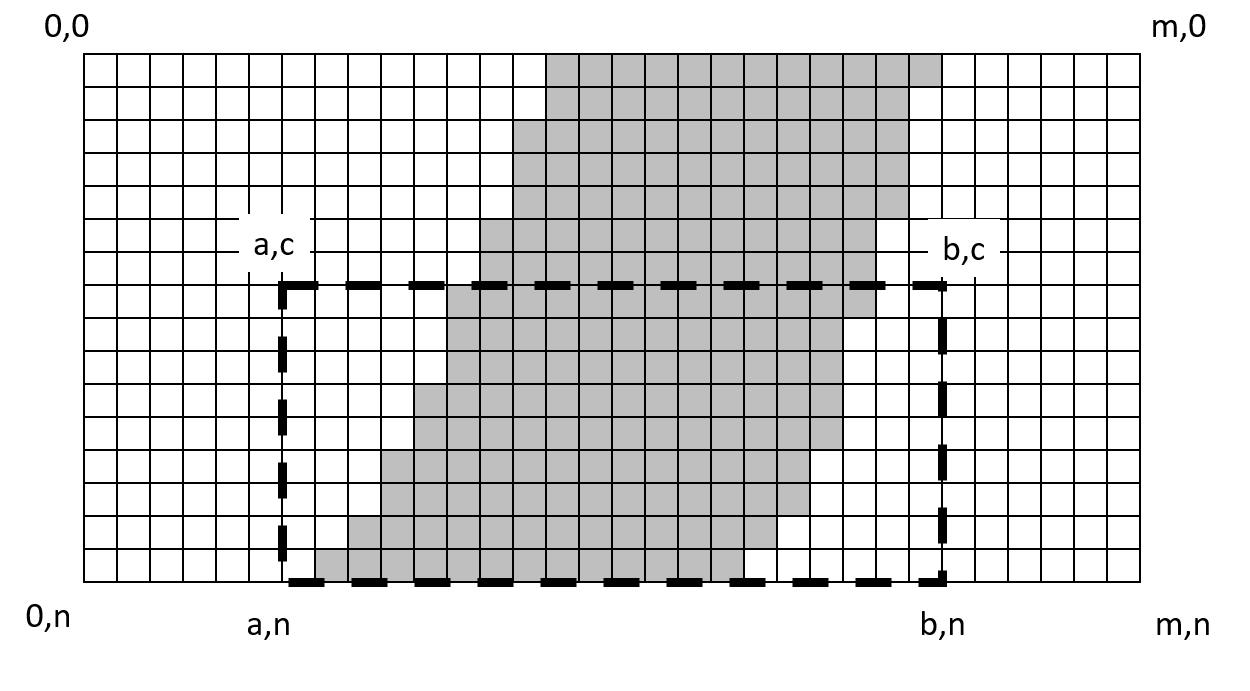
\includegraphics[width=3.0in]{pixelSubset}
%		\caption{Subset of pixels from the full image array}
%		\label{pixelSubset}
%	\end{figure}
%	
	
	
	\section{Development of binary edge map \textit{$E$}}
	
	 The binary edge map is developed using an edge detection algorithm. There are many of these but one the simplest involves filtering with a sobel operator. At the most basic level the Sobel operator is a 3x3 filter (or kernal) with positive coefficients on one side, negative coefficients on the other and zeroes in the middle. An example of a vertical line detection Sobel operator is below as equation \ref{sobelOp}. The binary edge map is created by taking the absolute value of the filtered result for each pixel and thresholding it over a certain value. For example if the absolute value of a filtered pixel is greater than 150, consider it an edge. \\

	\begin{equation}\label{sobelOp}
		\begin{bmatrix} 
		-1 & 0 & 1 \\ 
		2 & 0 & 2 \\ 
		1 & 0 & 1  
		\end{bmatrix}
	\end{equation}
	 	 
	 Applying a filter is similar to a form of 2D convolution. The filter is in the form of an odd dimensioned 2D array of coefficients. The central point of the filter is placed over the pixel being considered at $(x,y)$ and the value of the new pixel,  $(x',y')$ is the summation of all the elementwise products of the relevant coefficients of the filter and the corresponding image area. This occurs for all pixels in the image; it can be considered that the filter is `sliding' over the image pixel by pixel. As an example in figure \ref{filter}, a Sobel filter to detect vertical lines is being applied to example pixels. The top left pixel is in a region of change and would be considered an edge pixel after thresholding, note the value of the pixel is capped at a ceiling of 255 in this instance. The lower right pixel is in an area of relatively constant values and after thresholding would be not considered an edge.
	
	\begin{figure}
		\centering
		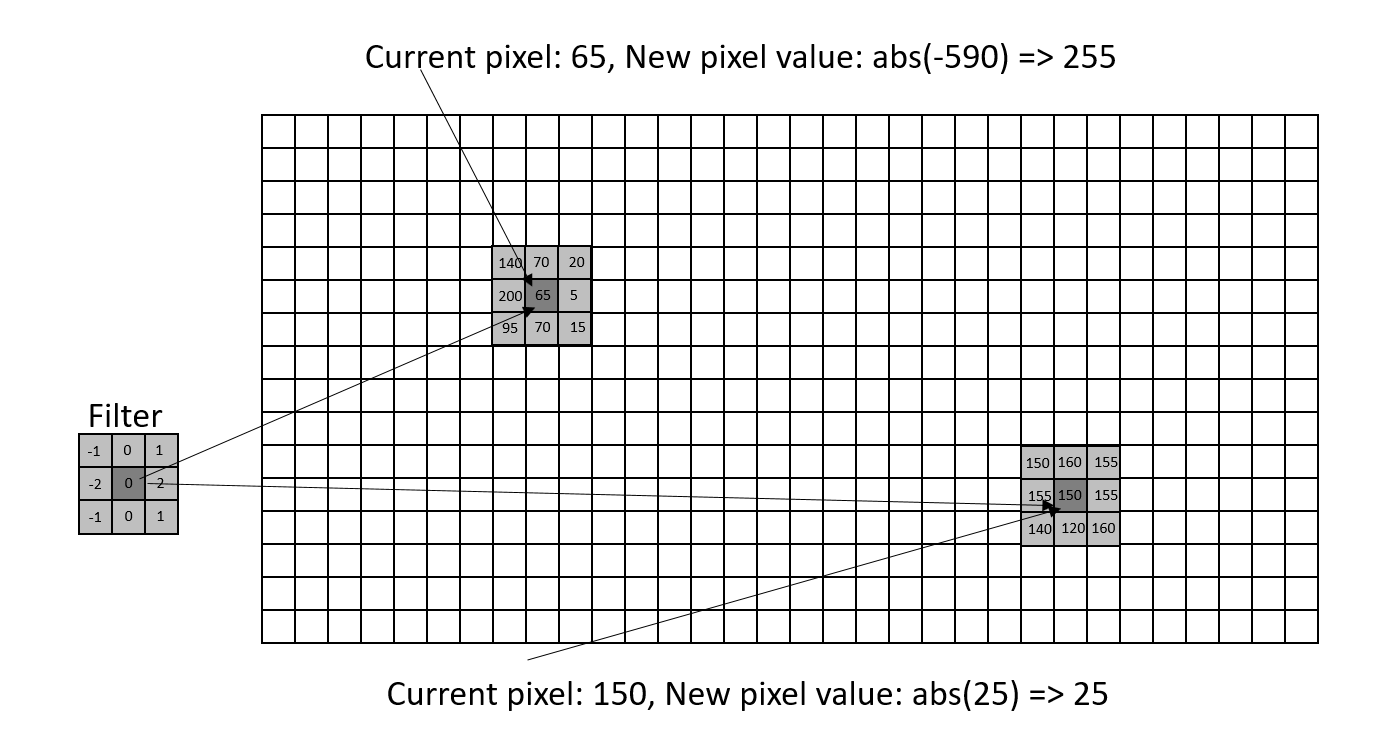
\includegraphics[width=5.0in]{filter}
		\caption{Example application of a filter to an arbitrary pixel}
		\label{filter}
	\end{figure}

	It is important to note that while the Sobel operator is a simple edge detection approach, this treatment has been at the most basic level. Horizontal and vertical kernals can be combined to develop a dual horizontal and vertical edge detector and a similar theory can be used to develop a detector sensitive to specific edge orientations. The Sobel operator approximates the gradient of the intensity thus the sign of the filtered output carries additional information that is not being considered here. Even so, one easy identifiable shortfall is the fact that regions of change over multiple pixels (`wide' edges) may produce multiple edge pixels after thresholding. The Canny Edge detector is an improved (albeit computationally slower) approach which includes non maximum suppression to develop a more refined edge map. These considerations are more complex and outside the scope of this brief overview.	
	
	
	\section{Line detection using Hough Transform}
		
	\begin{wrapfigure}{r}{0.35\textwidth}
		\begin{center}
			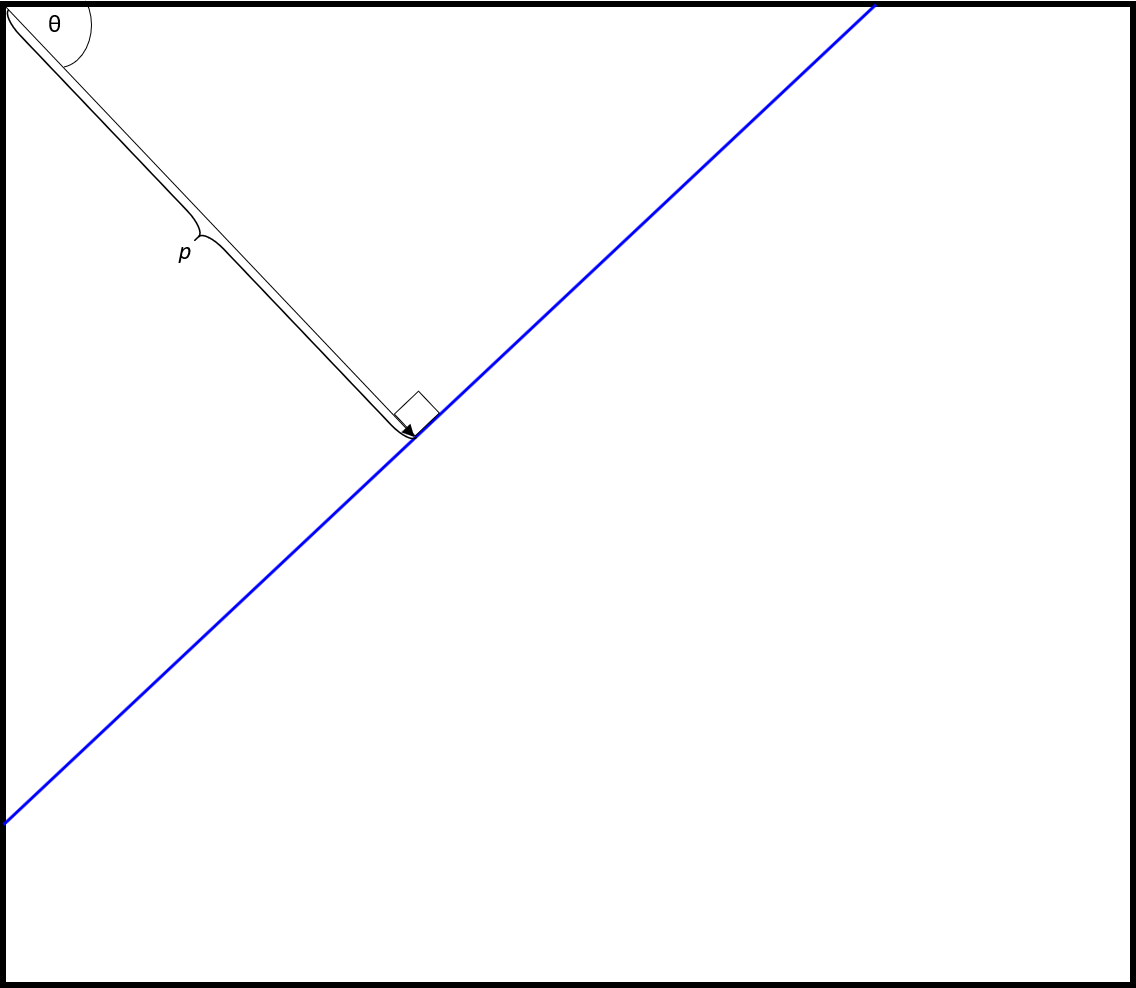
\includegraphics[width=0.34\textwidth]{HoughLineSpace}
		\end{center}
		\caption{Representation of an image line from $\rho$ and $\theta$ parameters}
		\label{HoughLineSpace}
	\end{wrapfigure}

	For the Hough transform we need to consider a line not in the standard form of $y = mx + c$ but being represented by the orientation, $\theta$, and length $\rho$ of a line from the image origin to the line along the line's normal vector. An outline of this representation is included as figure \ref{HoughLineSpace}. The Hough Transform maps cartesian coordinates $x, y$ into Hough space $\theta , \rho$ coordinates. 
%	
%	\begin{figure}
%		\centering
%		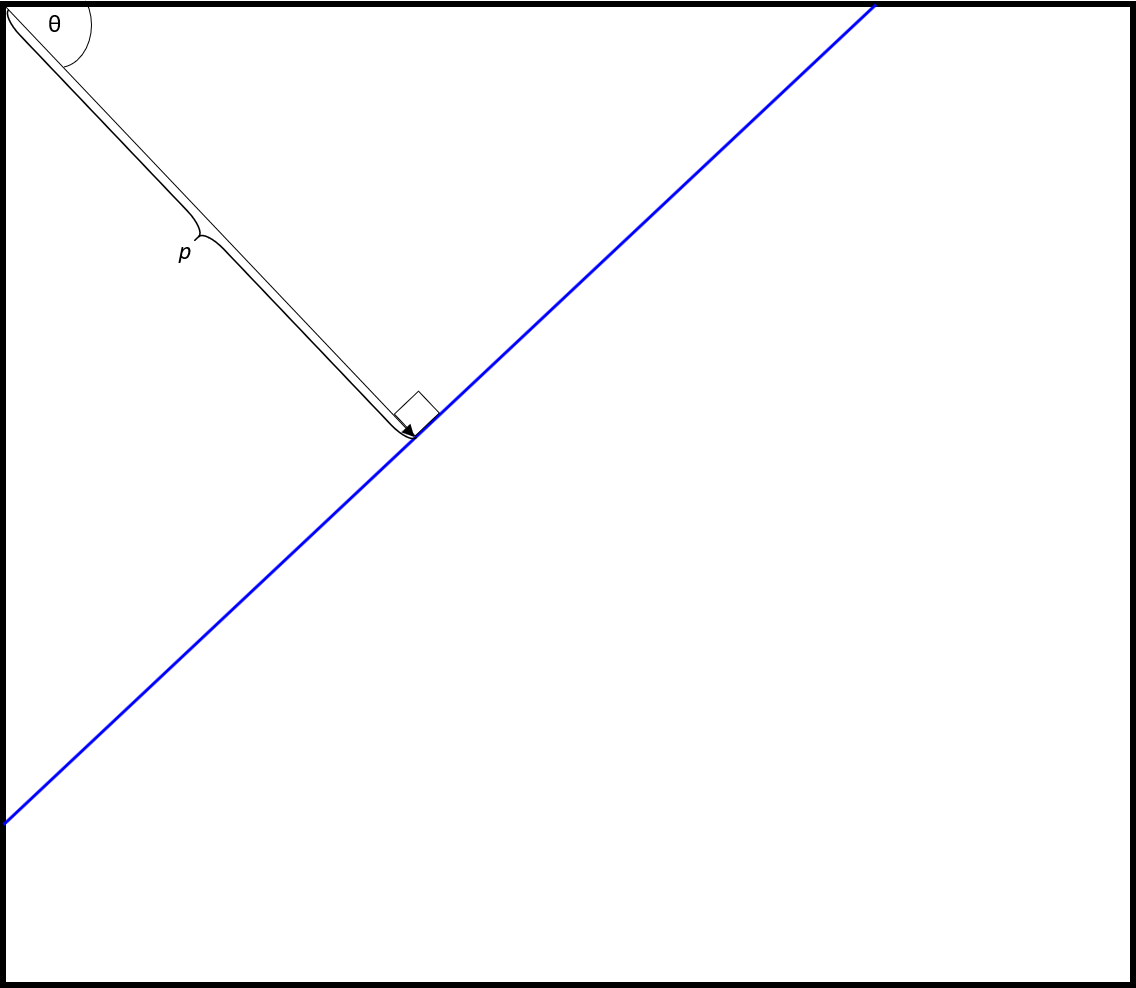
\includegraphics[width=3.0in]{HoughLineSpace}
%		\caption{Representation of an image line from $\rho$ and $\theta$ parameters}
%		\label{HoughLineSpace}
%	\end{figure}

	
	A single pixel in image space is represented as a single sinusiodal line in Hough space. This represents all the combinations of $\theta$ and $\rho$ that would result in a line passing through the pixel location in image space. Each point in Hough space is then considered as a `voting bin' where each pixel considered in the binary edge map `votes' for lines it could belong to. In the case of a single pixel, there would be one `vote' at each point in Hough space that the sinusiodal line corresponds to. This is demonstrated visually in figure \ref{HoughBasics}.
	
	\begin{figure}
		\centering
		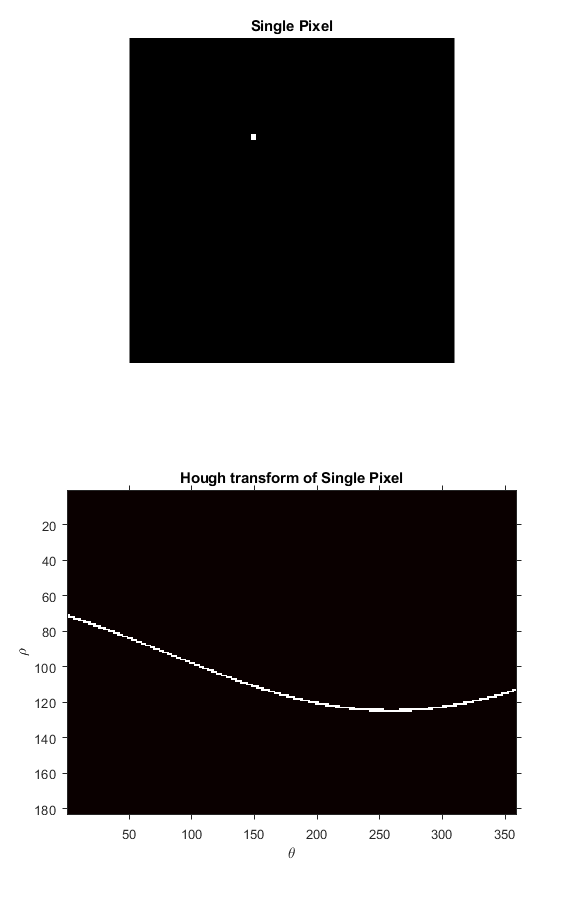
\includegraphics[width=3.0in]{HoughBasics}
		\caption{A single pixel in image space translating into a single sinusiodal line in Hough space}
		\label{HoughBasics}
	\end{figure}
	
%	\begin{wrapfigure}{R}{0.35\textwidth}
%		\begin{center}
%			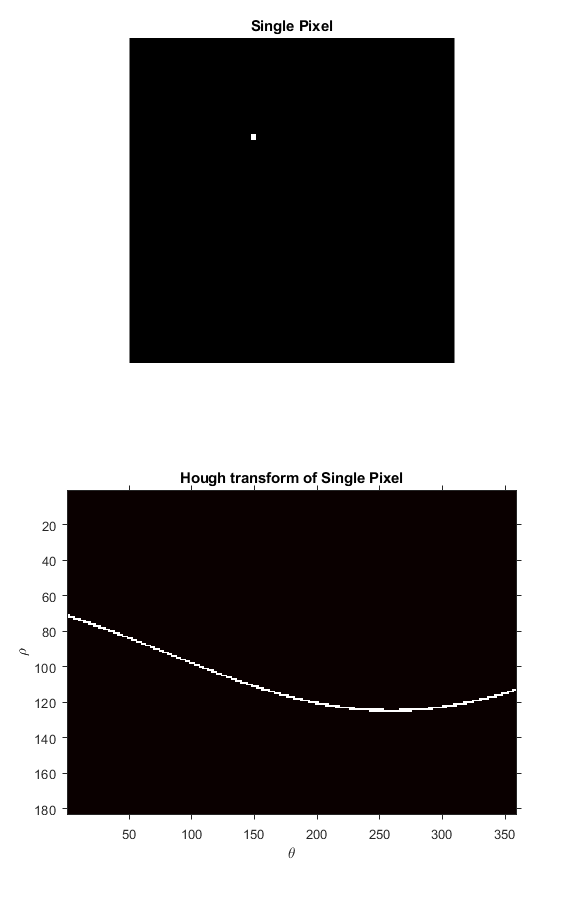
\includegraphics[width=0.34\textwidth]{HoughBasics}
%		\end{center}
%		\caption{A single pixel in image space translating into a single sinusiodal line in Hough space}
%		\label{HoughBasics}
%	\end{wrapfigure}
	
	If we then consider two pixels in image space, there is only a single possible line that could pass through both points. As per figure \ref{HoughBasics}, each individual pixel is transformed into a single line in Hough space but as there are two lines, there is a point where they intersect. This is demonstrated visually in figure \ref{HoughBasics2}. Investigating the Hough space `bins' would show multiple bins with a single vote (corresponding to the two sinusiodal Hough space lines) however one bin with two votes; ocurring at the location where the Hough space lines cross as both pixels place a `vote' at that location. This bin represents a peak in Hough space and corresponds to the $\theta$ and $\rho$ value which would result in a line passing through the two pixels.
	
	

%\begin{wrapfigure}{R}{0.35\textwidth}
%	\begin{center}
%		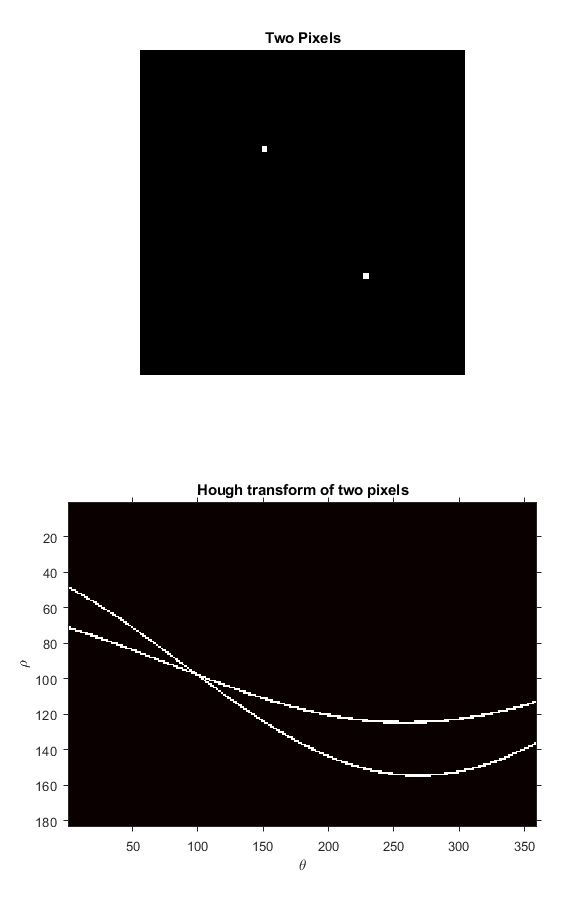
\includegraphics[width=0.34\textwidth]{HoughBasics2}
%	\end{center}
%	\caption{Two pixels in image space with intersecting Hough space lines}
%	\label{HoughBasics2}
%\end{wrapfigure}

	
	
	These examples are purely academic; the real power of the Hough transform comes where the input is a series of noisy edge pixels is provided as input. An indicative noisy edge map has been provided as input with the corresponding Hough transform in figure \ref{HoughDemoInput}. In this figure the intensity of the lines in the Hough transform represents the number of votes in each bin. The blue asterisks represent the local peaks above a certain threshold which indicate the detected lines.
	
	\begin{figure}
		\centering
		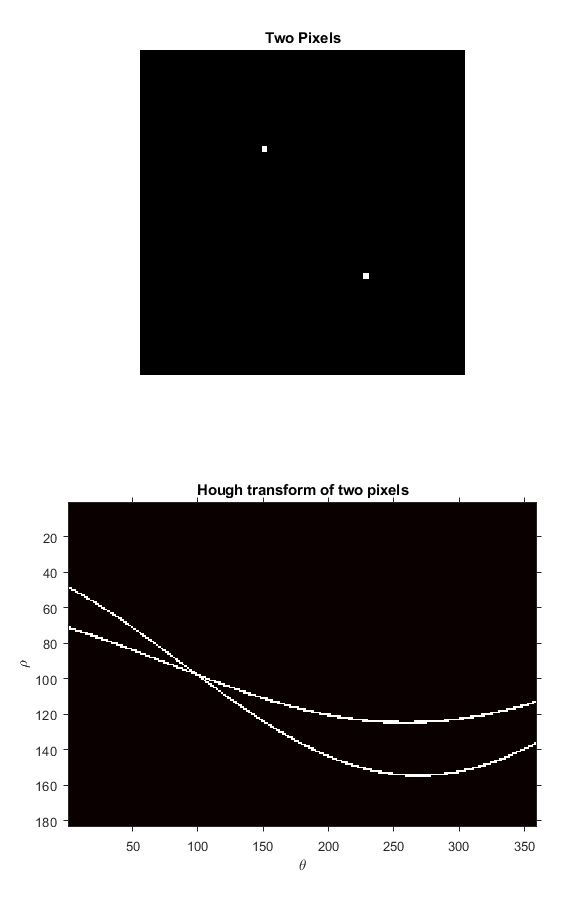
\includegraphics[width=3.0in]{HoughBasics2}
		\caption{Two pixels in image space with intersecting Hough space lines}
		\label{HoughBasics2}
	\end{figure}
	
	\begin{figure}
		\centering
		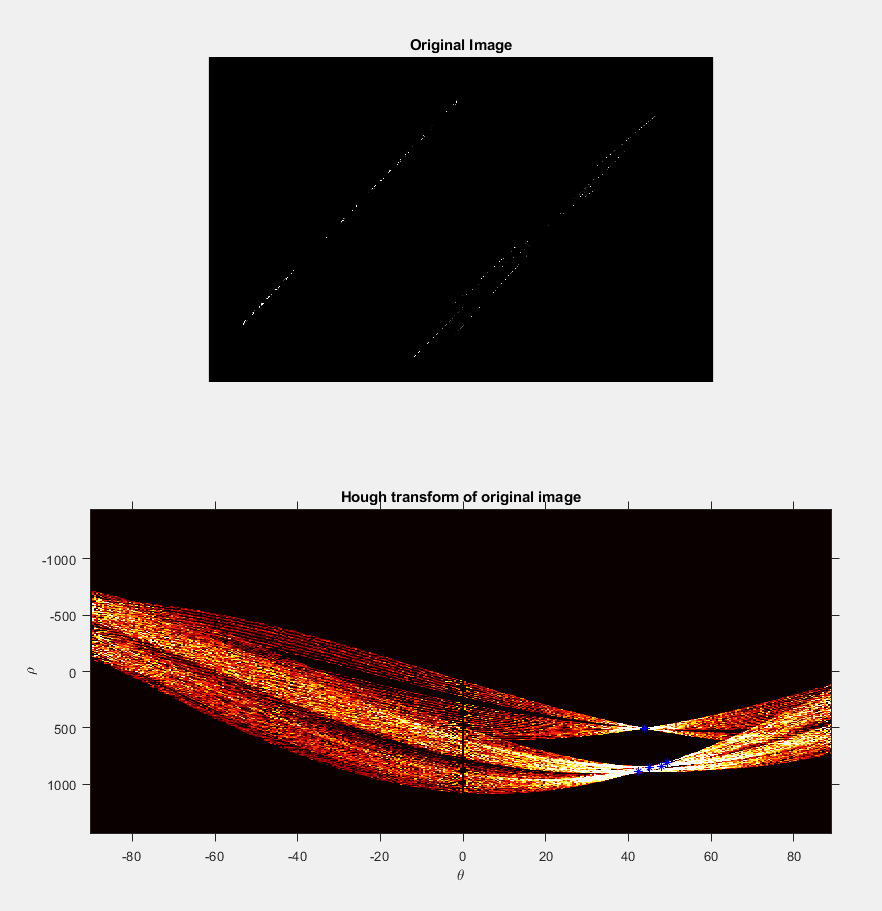
\includegraphics[width=3.0in]{HoughDemoInput}
		\caption{A representative binary edge map (top) and the relevant Hough transform (bottom)}
		\label{HoughDemoInput}
	\end{figure}

	
	The detected Hough lines can be transformed back into image space using the respective $\theta$ and $\rho$ values for the identified peaks. Figure \ref{HoughDemoOutput} shows the raw output of the detected lines as the left image showing multiple lines in close proximity. This is unsurprising given the multiple peaks detected as per figure \ref{HoughDemoInput}. Local non maximum supression means of all the lines in close proximity, only the maximum is considered and all other `close' lines are ignored. The output when this is applied is what we are after for our lane lines and is shown as the right hand image in figure \ref{HoughDemoOutput}.
	
	\begin{figure}
		\centering
		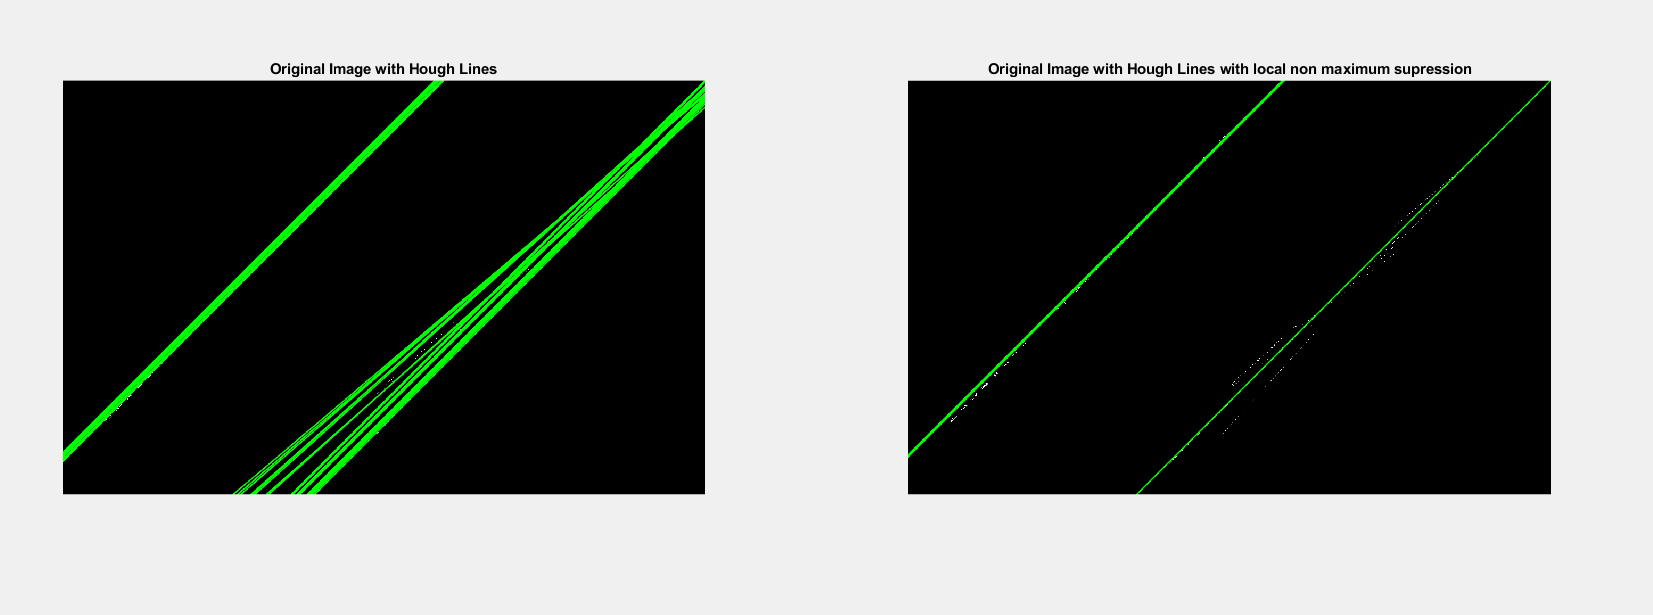
\includegraphics[width=5.0in]{HoughDemoOutput}
		\caption{Binary edge map from figure \ref{HoughDemoInput} with all detected edges (left) and with local non maximum suppression of lines (right)}
		\label{HoughDemoOutput}
	\end{figure}
	
	
	As with everything in this document, this has only been a superficial introduction to the Hough transform. The Hough transform has multiple tunable parameters such as the quantised resolution of $\theta$ and $\rho$ values and the thresholded vote count for a Hough peak to be considered a line. The intent of this document is merely for the reader to understand at a conceptual level how lane lines can be detected from the edge map so these aspects were not covered.
	
	
\end{document}